\documentclass[main.tex]{subfiles}
\begin{document}
\glsresetall

\section{Introduction}

In the \gls{lst}, the L1 trigger signal time must be be equalized throughout the whole camera. An L0 trigger signal which is transmitted from one module, will be propagated backplane to backplane from the center to the outer modules. To ensure that the L1 trigger time is the same in the whole camera, a series of delays must be applied in the backplanes, which depend on the distance of each module to the one propagating the signal. The requirement is that the time difference between all the camera modules must be lower than 300 ps. An algorithm for the time calibration was developed and tested at CIEMAT. A description of the time calibration procedure, algorithm and results on the tests carried on is included in this appendix.

\section{Time calibration procedure}

The time calibration is performed in cycles, where one module is the ''reference'' which distributes the signal (it is also the ''pulser'') and another module is the ''victim'', which receives the signal and must adjust a delay to be equalized with the previous module. The goal of the calibration is to set an outgoing delay ($oD^{V}$) and ingoing ($iD^{V}$) delay, in a way that the time for a signal to be transmitted from the central module to the victim ($t_{C}$), and from the victim to the center ($t_{L1}$) is the same as for the reference module. An scheme of the cycle is shown in picture \ref{fig:calibcicle}. 

\begin{figure}
  \centering
  \includegraphics[width=0.7\textwidth]{./Pictures/timecalib.pdf}
  \caption{Flux diagram of the calibration algorithm.}
  \label{fig:calibcicle}
\end{figure}

The delays are calculated determining the time difference between the L1 signal leaving the backplane, and the camera trigger signal returning to the backplane. These times are read from the difference between the TDC3 and TDC0 (time-to-digital converters) from the backplane. The calibration is separated in two phases, the ``down'' calibration and the ``up'' calibration, as shown in picture \ref{fig:calibcicle}.

\begin{itemize}

\item For the down calibration, the L1 signal distribution of the victim is deactivated, so the camera trigger signal is only triggered by the L1 of the reference. Because reference and victim are triggered by the same L0, the time at TDC0 for both modules will be the same. The difference $TDC3-TDC0 =\Delta$  can be measured both in the reference and victim modules, therefore the incoming delay is simply:
  \begin{equation}
    iD_{V} = (TDC3-TDC0)^{r}-(TDC3-TDC0)^{V} = \Delta^{R}-\Delta^{V}
  \end{equation}
  
  Once the required delay value is calculated, it is set in two steps: a coarse delay in steps of 10ns and a fine delay in steps of 36 ps.
  
\item For the up calibration, the L1 signal distribution of the victim is activated, and the one of the refence is deactivated. The goal of the up calibration is to set the outgoing delay in a way that the difference $(TDC3-TDC0)^V$, which is the total time the signal needs to go from the victim module to the center and back to the victim. The delay therefore is:

  \begin{equation}
    oD^{V} = L - (TDC3-TDC0)^V = L-\Delta^V
  \end{equation}
\end{itemize}

Where L is the latency, and corresponds to the $\Delta^{R}$ measured in the down calibration.
At the end of the cycle, the times $t_C$ and $t_{L1}$ will be the same both for reference and victim. At the start of the new cycle, the victim will be the new reference and other module is chosen as victim.\\
The calibration algorithm was implemented in a scripting language specifically designed for the communication with the different backplane registers.

\section{Time calibration setup and tests}

Two calibration setups were configured at CIEMAT, to implement the time calbration procedure. At first, four modules were set as shown in picture \ref{fig:timecalfig1}, allowing to run three time calibration cycles as described in the previous section. The test consisted in setting initial default values in the delays, given by the position of the modules, and running the calibration several times for different initial values to ensure the reliability of the procedure. After the success of the first implementation, a second setup was prepared involving eight modules. The calibration procedure was performed several times, to check the stability of the final TDC values and that the deviations with every backplane were in the allowed range of 300 ps.

\begin{figure}[!htb]
\minipage{0.5\textwidth}
\includegraphics[width=\linewidth]{Pictures/4modulessetupdiagram.pdf}
\endminipage\hfill
\minipage{0.5\textwidth}
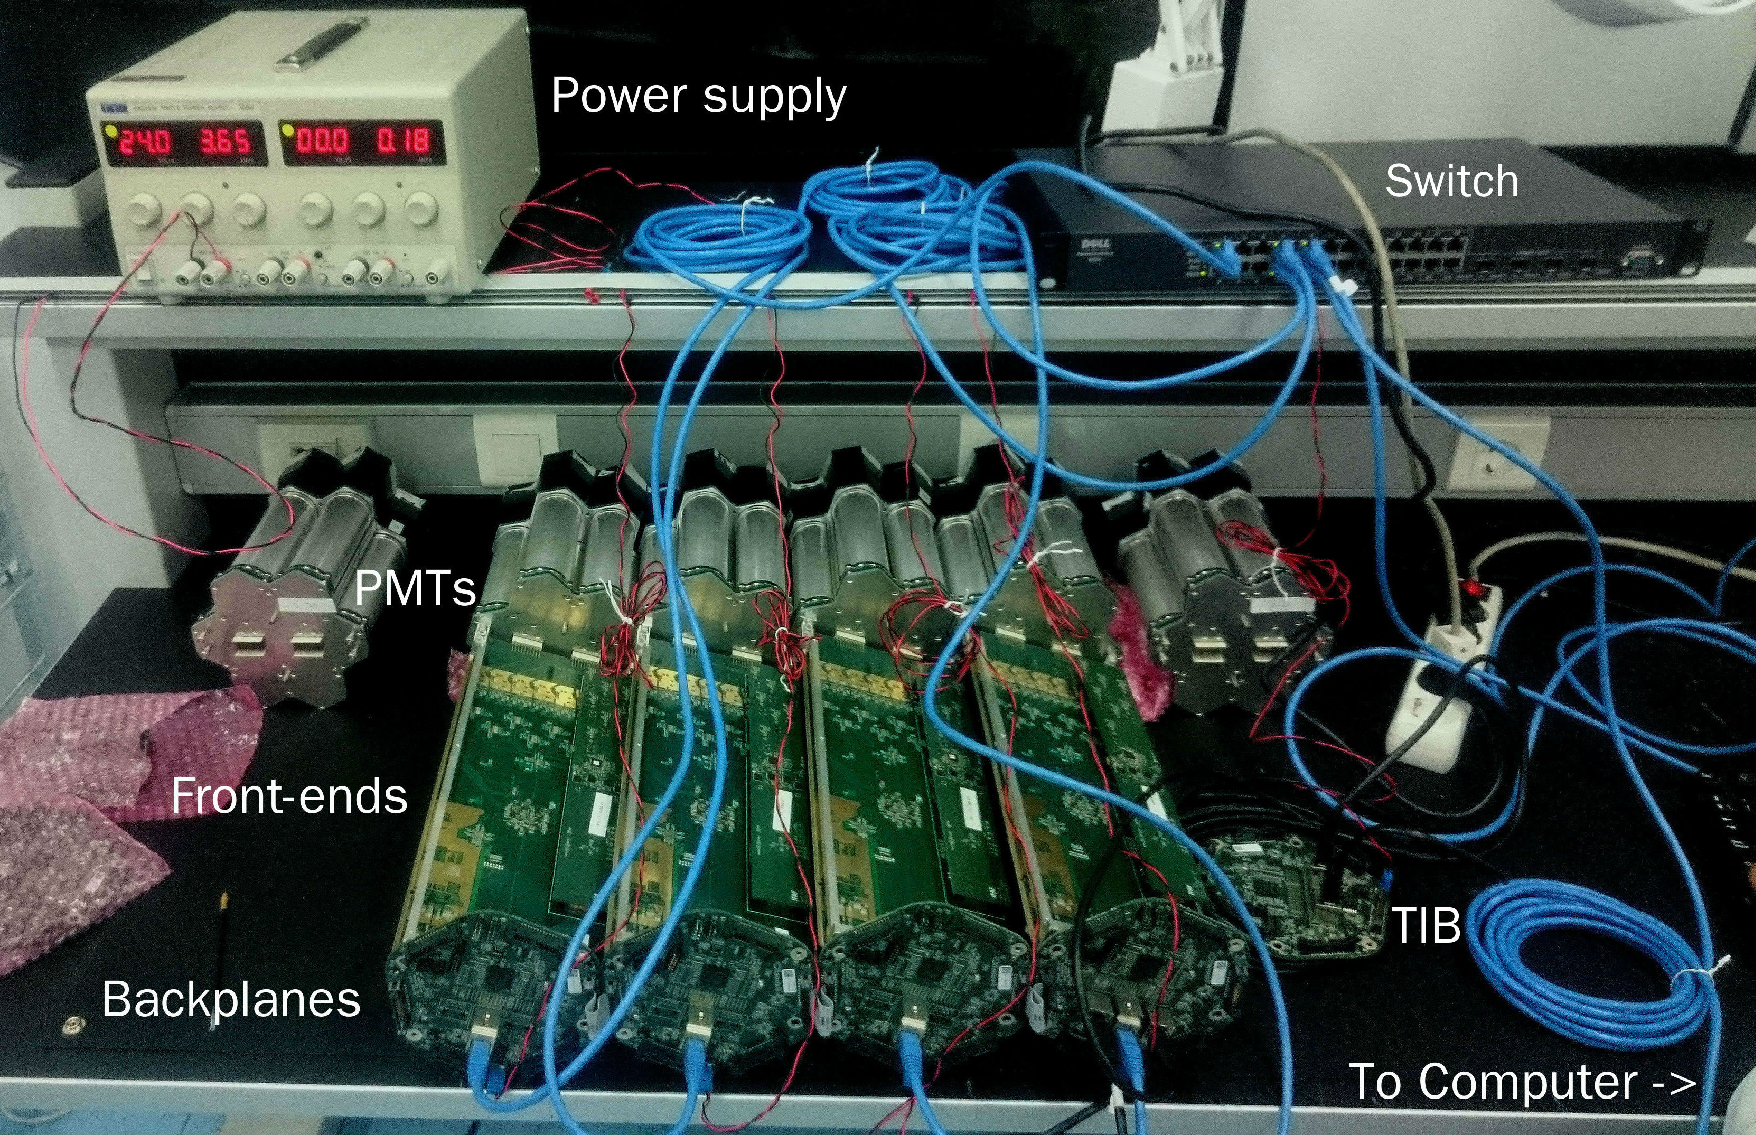
\includegraphics[width=\linewidth]{Pictures/4modulessetuppic.pdf}
\endminipage\hfill
\caption{\label{fig:timecalfig1}\textit{Left:} Diagram of the four modules setup. \textit{Right:} Picture of the actual setup at CIEMAT clean room.}
\end{figure}

Thanks to these two setups, the time calibration procedure was succesfully verified. The algorithm was then adapted to perform the calibration of the full camera, following the predefined paths of signal distribution as shown in picture \ref{fig:trigpaths}. This time calibration procedure must be run at last once every night of operation of the telescope.

\end{document}
